%!TEX root = main.tex
%\vskip -.75em
%\mypara{Summary}
% \jc{yet another QoE improvement doesn't sound very exciting}
User-perceived QoE (quality of experience) is a key driving force behind the ecosystem of web applications.
QoE depends critically on web page loading time, yet despite tremendous efforts to speedup page loading time,
%(\eg cutting tail latency via redundancy or pushing caches closer to end users), 
many users still suffer from suboptimal QoE.
%Unlike previous approaches such as cutting tails of response time or pushing caches closer to end users, 
This proposal introduces a new dimension for QoE optimization: harnessing the heterogeneity of {\bf QoE sensitivity to backend delay} across users. More importantly, such heterogeneity is prevalent even if the users request the same type of application/service.
%, \ie how sensitive a user's QoE is to the web backend delay.
For instance, a web request that has spent 50ms on wide-area networks before reaching the web server is much more likely to be affected by 10ms delay of the web service than a request that has already spent 500ms on the network. 
Such performance-induced discrepancy in QoE sensitivity is largely ignored in today's web services, but as we show, it has profound implications, especially when requests compete for limited resources.
In essence, web requests previously seen by the backend as identical can now be exploited to allocate resources efficiently by favoring requests whose QoE is more sensitive to the backend delay.
%We show early promising result that by making existing the web backend aware of QoE sensitivity, we could improve both QoE and resource efficiency than existing solutions.
In proposed work, we will investigate new opportunities to improve QoE and save resources by making web services aware of QoE sensitivity 
(\eg better scheduling policies and replica selection policies) and provide a technical roadmap to address the key challenges  (\eg estimating QoE sensitivity, and balancing fairness and efficiency).
% (1) We quantify its potential benefits in QoE and resource savings.
% (2) We propose novel algorithms for QoE-aware scheduling and resource allocation of web services. 
% (3) We present novel system designs and implement prototypes that make web services QoE-aware in practice.


% Thus, the goal of each subsystems in a large web service, such as web server or key-value store, should be to optimize the overall QoE of many users given limited resources. 
% A common approach to achieving this goal is for each subsystem to optimize some ``local'' performance metrics measured within its scope (\eg server-side delay) over all users, and the intuition is that if each subsystem follows the approach, it will optimize the overall QoE of users. 
% We argue, however, that this approach only achieves suboptimal QoE and can use more resources than necessary. 
% Our key observation is that {\em the impact of a subsystem's performance on a user's perceived QoE varies greatly among users} (modulo web page type, business relationship), so when sharing resources across users, each subsystem should take into account its impact on each user's QoE.
% One typical sources 
% This has profound implication on how web services should be optimized, and opens up many several new opportunities.


\section{Introduction}

% - QoE is important and our goal is to improve QoE for Web Services.
\noindent 
The fundamental challenge faced by large-scale web service providers (\eg Microsoft, Facebook, Google) is how to share resources of the web backend across users so as to optimize the user-perceived {\em QoE} (Quality of Experience). 
Web QoE has been shown to be critically dependent on web page loading time~\cite{??,??}.
Despite great amounts of efforts, ensuring desirable QoE is still an unsolved problem with \fillme\% users whose experience could have been improved from bad to good if the backend delay is zero~\cite{dqbarge}.

%Their business models, based on advertisement or subscription, are driven by user engagement, for which QoE is believed to play a vital role (among other factors such as content, user interfaces).

\mypara{Limitation of today's web backend}
Page load time, which we refer to as {\em end-to-end delay}, generally consists of three parts: client-side delay, wide-area network (WANs) delay, and backend delay.
%- Web services, like applications running in the cloud, have been basing their optimizations on the goal of improving server-side latency (sometimes the fraction of users meeting some fixed deadline)
%Because of the federated nature of Internet architecture, web service providers do not have full control over all types of delays.
%---to them, WANs and clients devices are largely blackboxes operated, not by the web services, but by ISPs, cellular carriers, and device vendors.
%(while web browsers and apps are developed by the web service providers, the client-side performance is largely decided by how OS share resources among multiple applications).
With web service providers only controlling the web backend, the performance metric they focus on optimizing is the 
%Thus, instead of optimizing for QoE directly, today's web services focus on reducing the 
%different requests have the same {\em QoE sensitivity to backend delay}
{\em backend delay}, under the assumption that a backend delay of $n$~ms has the {\em same} impact on any request.\footnote{Modulo the content-specific (\eg web page type) or user-specific (\eg free vs. premium subscription) factors.}
% That is, a backend delay of $n$~ms has the same effect on the QoE of any request.
For instance, they minimize the mean/tail backend delay or the fraction of requests whose backend delay exceeds some deadline (\eg 300ms).
%- This project takes a step back and asks a different question: does the latency have the same impact on user QoE? 
% In doing so, 
%all requests are optimized with the same objective function of backend response time; 
% an implicit assumption is that different requests have the same {\em QoE sensitivity to backend delay} (modulo content-/user-specific factors, such as web page type or subscription type, etc);
% that is, a backend delay of $n$~ms has the same effect on the QoE of different requests.

This proposal takes step back from this assumption, and ask {\em ``does each request really have the same sensitivity to backend delay?''}

%- The answer is no, which has profound impact on how web services should be built. [Give a simple example here.] In essence, this means giving each ``priority'', in terms of resources and scheduling, is cost-inefficient and suboptimal. [Give a simple example. resources wasted for users who are screwed already]
\mypara{Our insight} 
Our answer is {\em no}.  More importantly, even if the requests have no application-level differences (\eg web vs. video), such heterogeneous QoE sensitivity can still result from different non-backend delay (\eg wide-area network routing, client-side software)~\cite{timecard,dqbarge} across requests.
%Two observations contribute to this conclusion: the non-linear relationship between page load time and QoE~\cite{??} and the fact that the WAN/client delay varies among requests~\cite{timecard,dqbarge}, {\em the QoE sensitivity to backend delay varies among requests.}
For instance, a web request that has spent 50ms on wide-area networks before reaching the web server is more likely to be affected by 10ms delay of the web service than a request that has already spent 500ms on the network. 

The heterogeneous QoE sensitivity has profound implications for improving how web backend should allocate the limited resources among requests. 
By falsely assuming requests are equally sensitive to the backend delay, traditional web backend (Figure~\ref{fig:intro-overview}(a)) might waste precious resources (\eg wasting resources to optimize requests insensitive to the backend delay) and have suboptimal QoE (\eg spending inadequate resources on requests critically dependent on the backend delay). 
In contrast, the web backend should allocate resources smartly to each requests depending on their QoE sensitivity to the backend. 
On a message scheduling prototype, we found that such a QoE-driven scheduling policy can improve \fillme by \fillme\% over a baseline first-come-first-serve policy.
%\jc{bring up some concrete improvement numbers}
%\jc{need to highlight that this is not because application differents}

\begin{figure}[t]
	\centering
	\vspace{-0.5cm}
	\hspace{0.6cm}
	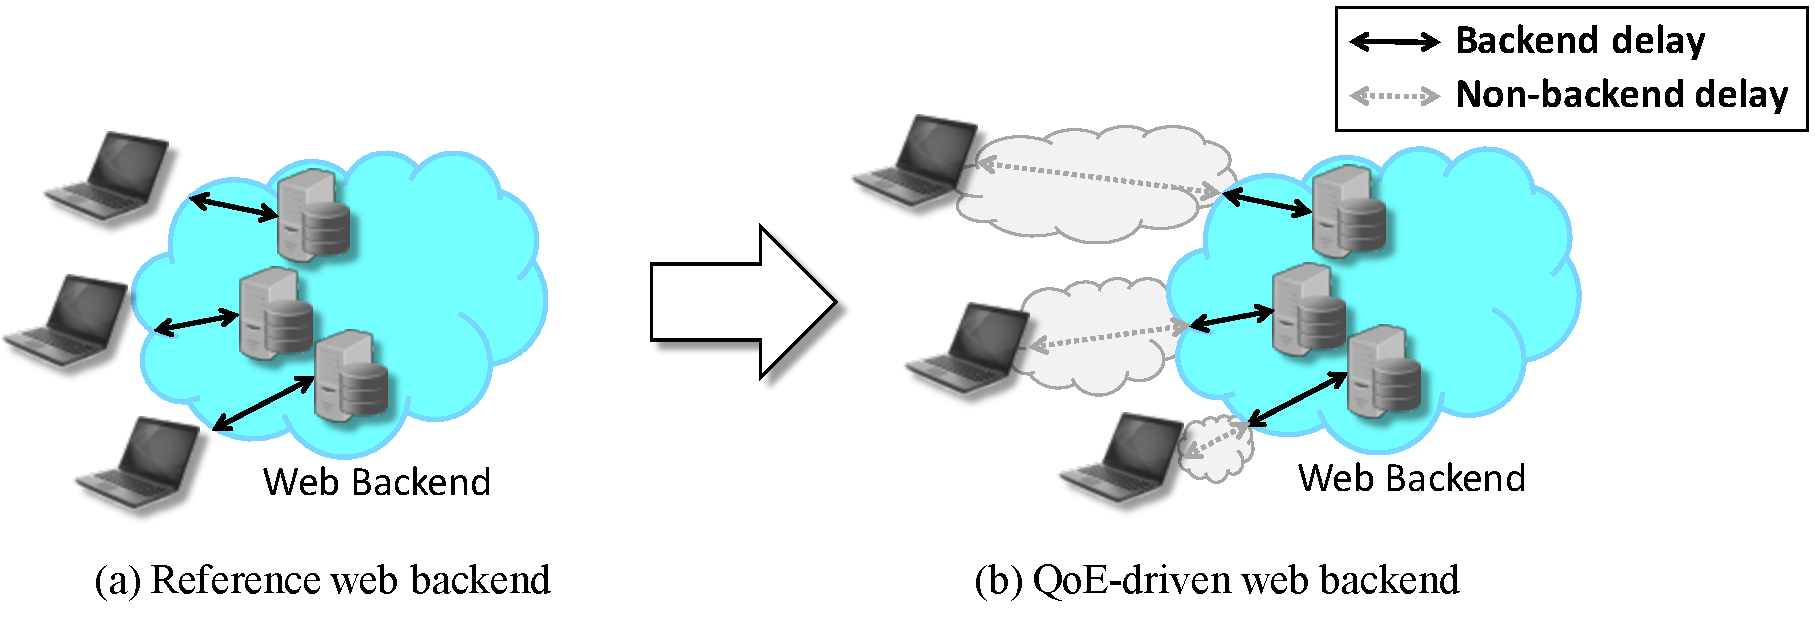
\includegraphics[width=0.95\textwidth]{figs/intro-overview.pdf}
	\vspace{-0.3cm}
	\caption{We propose to re-architect (a) the reference web backend which seeks to minimize the backend delays into (b) the QoE-driven web backend which seeks to minimize the impact of backend delay on user-perceived QoE.}
	\label{fig:intro-overview}
\end{figure}

%\jc{give a figure to contrast optimization of backend in-isolation vs. QoE-aware.}

%- Research goal: This project proposes that the web service backend should be aware of the QoE sensitivity. This effectively changes how one formulates the web service optimization problem.
\mypara{Research plan}
This proposal introduces ``QoE sensitivity'' as a new dimension for QoE optimization of web backends. 
Through developing novel algorithms and architectural components, we show that a {\bf QoE-driven web backend} (Figure~\ref{fig:intro-overview}(b)), which is aware of and exploits the differences of QoE sensitivity across requests, can substantially {\em improve the resource/QoE tradeoffs} of web service backend; \ie better QoE without using more resources, or saving resources without degrading QoE. 
% Note that being QoE sensitivity does not require expensive infrastructure changes (\eg adding hardware or changing software stack).
We divide the proposed research into four tasks.
%We use the following roadmap to thoroughly examine the benefits and challenges of QoE-sensitivity-aware web service backend.

\begin{packeditemize}
\item{\bf Quantifying potential benefits (Task \#1).}
We will design and carry out measurement studies to quantify the various improvements brought by QoE-driven web backend in the wild. We will provide a taxonomy of use cases of QoE-driven control in different aspects of today's web backend. We will also use large dataset from commercial web services to help understand opportunities in the actual traffic pattern in real world.

\item{\bf QoE-driven control algorithms (Task \#2).}
We will develop and build prototype of novel QoE-driven control policies for web backend, including resource allocation, message scheduling, and replica selection. Our design goals are (1) that the policies should balance near-optimal QoE and efficiency (minimal overhead of decision-making), and (2) that the implementation of these policies should be amenable to existing systems (\eg only control-plan changes).

\item{\bf QoE-driven backend architectural (Task \#3).}
We will develop new architectural component of web backend, including tracing infrastructure and QoE prediction models, to estimate the QoE sensitivity of requests in real-time. In the process, we will investigate the possibility of incremental deployment through reusing the existing tracing and telemetry infrastructure in large-scale web backends as much as possible.

\item{\bf Impact on QoE fairness (Task \#4).}
Finally, we will explore appropriate definitions of fairness to characterize the outcome of QoE-driven web backend. This would help us strike a desirable balance between QoE-driven optimization and QoE fairness. This would also help us recognize potential threads of other systems/users taking advantage of the QoE-driven policies of the backend.

\end{packeditemize}


%\jc{why these applications?}

%\jc{Common challenges! getting QoE sensitivity, fairness definition!}

\mypara{PI qualification}
The PI's expertise includes computer networking, Internet QoE, and data analytics systems.
He has published 11 peer-reviewed research papers (6 first-authored) in top-tier networking and system conferences (\ie SIGCOMM, NSDI, CoNEXT).
More importantly, the PI has a deep understanding of Internet QoE. His doctoral dissertation, titled ``Enabling Data-Driven Optimization of Quality of Experience in Internet Applications'', is among the first systematic studies to apply data-driven approach to improving Internet application QoE. The dissertation won the CMU SCS Doctoral Dissertation Award and was nominated for ACM Dissertation Award.
During his PhD and postdoctoral years, he has extensive collaborations with the industry, including Microsoft Research, Conviva Inc., and Google Research. These strong connections will help the proposed research to gain insights from the industry and provide viable path for deployment.


% \vspace{0.2cm}
% \noindent{\em Thrust \#1: How much potential benefit can we get?}

% \vspace{0.2cm}
% \noindent{\em Thrust \#2: How to re-architect web services to be QoE-aware?}

% \vspace{0.2cm}
% \noindent{\em Thrust \#3: How to propagate user-perceived QoE information?}

%- This project proposes to re-architect the web service backend by making it QoE-aware. Our roadmap has three steps.\\
%1. XXX\\
%2. YYY\\
%3. ZZZ



% \vspace{2cm}
% User-perceived quality of experience (QoE) is one of the driving forces behind the Internet ecosystem, which consists of {\em subsystems}, \eg datacenters, CDNs, cellular carriers, backbone networks, content providers, who share resources across users. 
% % End-to-end Quality of Experience (QoE) is the driving force behind today's Internet application ecosystem, which includes several subsystem
% % The Internet application ecosystem consists of many subsystems, Cloud, ISP, CDNs, etc, and 
% Thus, one fundamental question is {\em how to share resources across users in a way that optimizes their overall QoE?}
% The primary constraint is that these subsystems are {\em federated}: it is impractical to orchestrate a global optimization where they relinquish the control on how their resources are shared. 
% Instead, the conventional wisdom has been that each subsystem shares its resources among users in a way that optimizes the overall performance metrics within its limit and imposes no differentiation between users if they are ``functionally'' identical (\ie same service, business relationship, etc).

% In contrast, we are driven by a simple observation derived directly from the federated nature of the Internet ecosystem.
% In a subsystem, there is {\em a substantial heterogeneity} among its users with respect to how sensitive their QoE is to the performance of the subsystem, even if these users are functionally identical. 
% Thus, the right question to ask is {\em not} how a subsystem should optimize the overall performance among users; instead, it should minimize {\em overall impact on user-perceived QoE}, which requires treating users differently, rather than equally, depending on how much impact it has on the user's perceived QoE.

% In this proposal, we apply this idea to improving QoE of web services.

% \mypara{Research goals}

% \noindent {\bf Intellectual Merit.~~}
% This proposal applies this idea in the context of cloud services. 
% \jc{what it means to cloud services? requests are going to be treated differently, etc} 
% Specifically, this idea can be applied to many services inside a cloud. \jc{talk about more applications}
% In this project, we plan to answer three key question:

% First, how much potential benefit does this idea have?

% Second, how to design a QoE-aware cloud scheduling/resource allocation mechanism?

% Third, how to propogate QoE information from users to the cloud?

% \noindent {\bf Broader Impacts.~~}


% \noindent {\bf Keywords.~~} 



% QoE matters to everyone!

% \subsection{Missed Opportunities}
% \begin{itemize}

% \item Today's tenant: every user should be treated with the same performance goal. Implicit assumption is that the impact of a subsystem is the same on all users.

% \item However, the federated architecture means:\\
% 1. QoE can be affected by any subsystem\\
% 2. Each subsystem serves users with different QoE sensitivities.

% \item Fundamental mismatch: some users who are less sensitive to the subsystem get over-optimized, while others who are more sensitive to the subsystem get under-optimized.

% \item New approach: minimize the overall impact on QoE. 

% \end{itemize}

% \subsection{This proposal: Making Cloud QoE-Aware}
% \begin{itemize}

% \item How the cloud works today -- agnostic to QoE

% \item QoE curve

% \item Examples of how things can be done differently!

% \end{itemize}


% \subsection{Research Roadmap:}
% \begin{itemize}

% \item How much potential benefit does this idea have?

% \item How to design a QoE-aware cloud scheduling/resource allocation mechanism?

% \item How to propagate QoE information from users to the cloud?

% \end{itemize}
